\subsection{PID Controller}
    %\subsubsection{Components}
        $u(t) = e^{st}$, dependence of (t) left out for shortness\\
        \begin{minipage}{0.28\linewidth}
            \titel{proportional}
            \begin{align*}
                y = k \cdot u
            \end{align*}
        \end{minipage}
        \begin{minipage}{0.32\linewidth}
            \titel{Differentiator}
            \begin{align*}
                y = \frac{du}{dt} = s \cdot u
            \end{align*}
        \end{minipage}
        \begin{minipage}{0.32\linewidth}
            \titel{Integrator}
            \begin{align*}
                y = \int u dt = \frac{1}{s} u
            \end{align*}
        \end{minipage}
        %\newcolumn
        
    %\subsubsection{Characteristics of P, PI, PD and PID}
    
    \titel{PI-Controller ($\propto$ accumulated error)}
        \begin{minipage}{0.49\linewidth}
            \begin{align*}
                PI(s) = k_P \frac{(s + \frac{k_I}{k_P})}{s}
            \end{align*}
            - $e_{\text{ss}} = 0$ for step input\\
            $k_I$ increases:\\
            - more oscillatory response\\
            - noise sensitivity doesn't change
            %\begin{itemize}
            %    \item $e_{\text{ss}} = 0$ for step input
            %    \item $k_I$ increases:
            %    \begin{itemize}
            %        \item more oscillatory response
            %        \item noise sensitivity does not change
            %    \end{itemize}
            %\end{itemize}
        \end{minipage}
        \begin{minipage}{0.49\linewidth}
            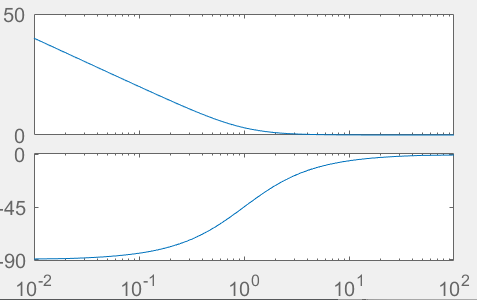
\includegraphics[width = \linewidth]{src/images/PI-controller.png}
        \end{minipage}

    \titel{PD-Controller ($\propto$ rate of change of error)}
        \begin{minipage}{0.49\linewidth}
            \begin{align*}
                PD(s) = k_D (s + \frac{k_P}{k_D})
            \end{align*}
            - acts like damping\\
            $k_D$ increases:\\
            - $e_{ss}$ unaffected\\
            - less oscillatory, maybe slower\\
            - increased sensitivity to noise\\
        \end{minipage}
        \begin{minipage}{0.49\linewidth}
            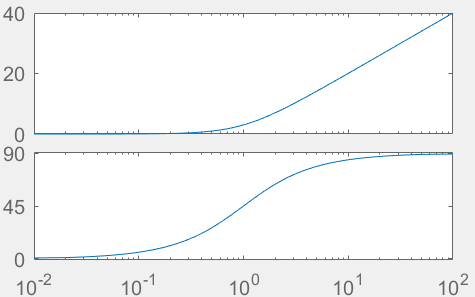
\includegraphics[width = \linewidth]{src/images/PD-controller.png}
        \end{minipage}
    
    \titel{PID-Controller}
        \begin{minipage}{0.49\linewidth}
            \begin{scriptsize}
                \begin{align*}
                    &C_{\text{PID}}%= k_P + \frac{k_I}{s} + k_D \cdot s\\
                    = \frac{k_P \cdot s + k_I + k_D \cdot s^2}{s}\\
                    &= k_P(1 + \frac{1}{T_I \cdot s} + T_D \cdot s)\\
                    %k_P &= \text{Proportional gain}\\
                    %k_I &= \text{Integral gain}\\
                    %k_D &= \text{Derivative gain}\\
                    T_I &= \text{Integral time constant gain}\\
                    T_D &= \text{Derivative time constant}
                \end{align*}
            \end{scriptsize}
        \end{minipage}
        \begin{minipage}{0.49\linewidth}
            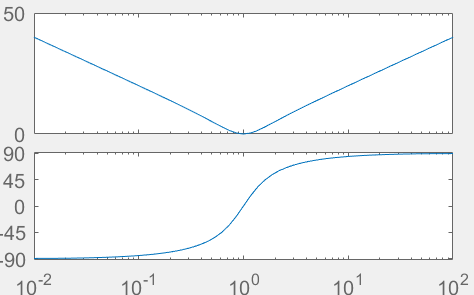
\includegraphics[width = \linewidth]{src/images/PID-controller.png}
        \end{minipage}

    \titel{P-Controller ($\propto$ error)}
        $k_P$ increases:\\
        - closed-loop of 2nd+ order more oscillatory, remain stable\\
        - $e_{ss}$ decreases\\
        - faster response\\
        - increased sensitivity to noise

